\documentclass{article}
\usepackage[nl]{../personal-packages/thomaspackage-obsolete}
\usetikzlibrary{matrix}

\begin{document}
    \tableofcontents
    \newpage

    \section{Limieten}\label{sec:limieten}
    Onthoud
    \begin{align*}
        &\lim_{x\to 0} \frac{x}{\sin x} = 1 \\
        &\lim_{n \to \infty} \left( 1 + \frac a n \right)^n = e^a \\
        &\lim_{n \to \infty} \sqrt[n]{n} = 1 \\
    \end{align*}
    \[
        f(h) \in o(h) \text{ als } \lim_{h \downarrow 0} \frac{f(h)}{h} = 0.
    \]
    \section{Sommen}\label{sec:sommen}
    Onthoud
\begin{align*}
    \sum_{k=c}^{\infty} r^k &= \frac{r^c}{1-r} \text{ als $|r|<1$}\\
    \sum_{k=1}^{\infty} \frac{1}{k^2} &= \frac{\pi^2}{6} \\
    \sum_{k=0}^\infty \frac{x^k}{k!} &= e^x \\
    \sum_{k=0}^n \binom{n}{k} a^k b^{n-k} &= (a+b)^n \\
    \sum_{i=1}^n i &= \frac{n(n+1)}{2} \\
\end{align*}

Uit de eerste kunnen we andere sommen afleiden.
bijvoorbeeld
$\displaystyle \sum_{k=0}^{\infty} kr^k $ of $\displaystyle \sum_{k=0}^{\infty} (k+1)r^k: $
\begin{align*}
    \sum_{k=0}^{\infty} r^k &= \frac{1}{1-r} \text { differenti\"eren aan beide kanten } \to \\
    \iff \sum_{k=1}^{\infty} kr^{k-1} &= \frac{-1}{(1-r)^2} \\
    \iff \sum_{k=0}^{\infty} kr^k &= \frac{-r}{(1-r)^2} \quad \text{of index verschuiven:} \\
    \iff \sum_{k=0}^{\infty} (k+1)r^k &= \frac{-1}{(1-r)^2} \\
\end{align*}

Dit kunnen we natuurlijk voortzetten door nog een afgeleide te nemen, dan krijgen we
\begin{align*}
    \sum_{k=1}^{\infty} kr^{k-1} &= \frac{-1}{(1-r)^2} \\
    \iff \sum_{k=2}^\infty k(k-1) r^{k-2} &= \frac{2}{(1-r)^3} \\
    \iff \sum_{k=0}^\infty \frac{(k+1)(k+2)}{2} r^k &= \frac{1}{(1-r)^3}.
\end{align*}

Merk op dat
\begin{align*}
    \binom{-3}{n} (-1)^n &= (-1)^n \frac{(-3)(-4)\dots (-3-n+1)}{n!} \\
    &= \frac{3 \cdot 4 \dots (n+2)}{n!} \\
    &= \frac{1}{2} \frac{(n+2)!}{n!} \\
    &= \frac{(n+2)(n+1)}{2}.
\end{align*}

Hier worden we blij van, want eigenlijk is $\frac{1}{(1-r)^n} $ het binomium van Newton
\[
    (1+x)^\alpha = \sum_{k=0}^\infty \binom{\alpha}{k} x^k
\]
die we af kunnen leiden (idee van Newton) uit de formule voor $(a+b)^n$ door $a=1$ en voor $n$ een getal $\alpha \in \reals$ in te vullen.

Nu kunnen we ook $\displaystyle \sum_{k-1}^\infty \frac{1}{k} r^k$, bijvoorbeeld $\displaystyle \sum_{k=1}^{\infty} \frac{1}{k2^k}$:
\begin{align*}
    \sum_{k=0}^{\infty} r^k &= \frac{1}{1-r} \text { integreren aan beide kanten } \to \\
    \iff \sum_{k=0}^{\infty} \frac{1}{k+1} r^{k+1} &= -\log_e (1-r) \\
    \iff \sum_{k-1}^\infty \frac{1}{k} r^k &= \log_e (\frac{1}{1-r})
\end{align*}

Eindige sommen kunnen we nu ook, \textbf{deze formule geldt algemener voor $r\neq 1$} omdat dit een eindige som is en dus altijd een waarde heeft, maar dan is de afleiding natuurlijk anders.
\begin{align*}
    \sum_{k=c}^n r^k &= \sum_{k=c}^\infty r^k - \sum_{k=n+1}^\infty r^k
\end{align*}

\subsection{Producten van sommen}\label{subsec:producten}

\begin{align*}
    \left( \sum_{k=0}^\infty a_k x^k \right) \left( \sum_{\ell=0}^\infty b_\ell x^\ell \right) &= \sum_{n=0}^\infty \sum_{k+\ell =n} a_k b_\ell x^{k+\ell} \\
    &= \sum_{n=0}^\infty \sum_{k=0}^n a_k b_{n-k} x^n = \sum_{n=0}^\infty c_n x^n.
\end{align*}

    \section{Taylorreeksen}\label{sec:taylorreeksen}
    \subsection{Standaard Taylorreeksen}\label{subsec:standaardTaylorreeksen}
Onthoud: de cosinus is even (symmetrisch rond de $y$-as) en deze heeft even machten, evenzo is de sinus oneven.
De standaard Taylorreeksen rond 0 om te onthouden zijn
\begin{align*}
    \cos x &\coloneqq \sum_{n=0}^\infty (-1)^n \frac{x^{2n}}{(2n)!} \\
    \sin x &\coloneqq \sum_{n=0}^\infty (-1)^n \frac{x^{2n+1}}{(2n+1)!} \\
    e^x &\coloneqq \sum_{n=0}^\infty \frac{x^n}{n!} \\
    \ln (1+x) &= \sum_{n=0}^\infty (-1)^{n} \frac{x^{n+1}}{n+1} \\
    \arctan x &= \sum_{n=0}^\infty (-1)^n \frac{x^{2n+1}}{2n+1} \\
\end{align*}
De reeks van $\sqrt{1+x}$ kun je vinden door te stellen
\begin{align*}
    \left( c_0 + c_1 x + c_2 x^2 + \dotsm \right)^2 &= 1+x \\
    c_0^2 + 2 c_0 c_1 x + \dotsm &= 1+x
\end{align*}
waaruit de eerste paar termen snel te vinden zijn, namelijk $c_0=1$ en dus $c_1 = \frac 1 2$ enzovoorts.

Merk op dat inderdaad
\[
    \ln \left(1 + \frac a n \right)^n = n \ln \left(1 + \frac a n \right) = n \left(\frac a n - \frac{a^2}{2n^2} + \dots \right) \upto{n \to \infty} a.
\]
\subsection{Gonioformules} \label{gonioformules}
\subsubsection{Waardes van de sinus en de cosinus}
\begin{figure}[h!]
    \centering
    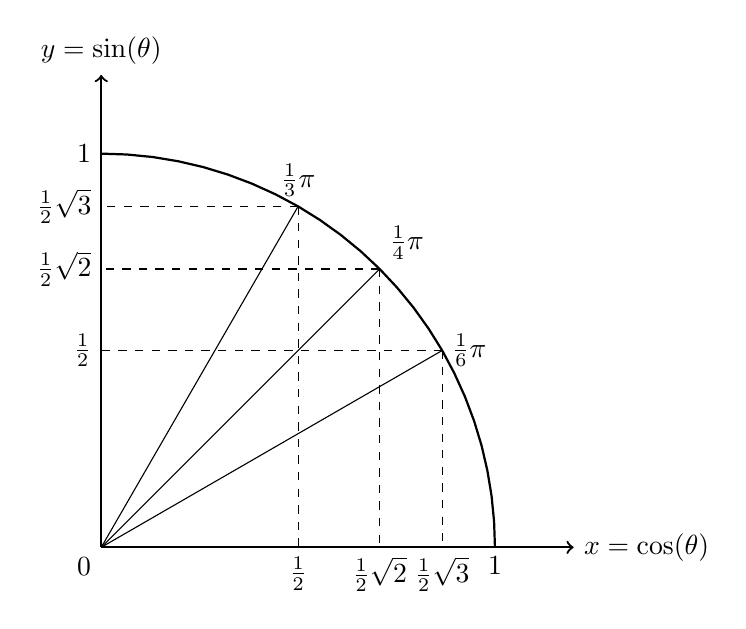
\begin{tikzpicture}[scale=5]
        \draw (1,0) node [below] {1};
        % assen
        \draw [->, thick] (0,0) -- (1.2,0) node [right] {$x = \cos(\theta)$};
        \draw [->, thick] node [below left] {0} (0,0) -- (0,1.2) node [above] {$y = \sin (\theta)$};
        % kwart cirkel
        \draw [thick,domain=0:90] plot ({cos(\x)}, {sin(\x)}) node [left] {1};
        % driehoeken
        \draw (0,0) -- (.866, .5) node [right] {$\frac{1}{6} \pi$};
        \draw [dashed] (.866, .5) -- (.866, 0) node [below] {$\frac{1}{2} \sqrt{3}$};
        \draw [dashed] (.866, .5) -- (0, .5) node [left] {$\frac{1}{2}$};
        \draw (0,0) -- (.707, .707) node [above right] {$\frac{1}{4} \pi$};
        \draw [dashed] (.707, .707) -- (.707, 0) node [below] {$\frac{1}{2} \sqrt{2}$};
        \draw [dashed] (.707, .707) -- (0, .707) node [left] {$\frac{1}{2} \sqrt{2}$};
        \draw (0,0) -- (.5, .866) node [above] {$\frac{1}{3} \pi$};
        \draw [dashed] (.5, .866) -- (.5, 0) node [below] {$\frac{1}{2}$};
        \draw [dashed] (.5, .866) -- (0, .866) node [left] {$\frac{1}{2} \sqrt{3}$};
    \end{tikzpicture}
\end{figure}

\subsubsection{Verdubbelingsformules}

De verdubbelingsformules kunnen we afleiden met behulp van e-machten.
We gebruiken
\begin{align*}
    \cos x = \frac 1 2 \left( e^{ix} + e^{-ix} \right) \\
    \sin x = \frac 1 {2i} \left( e^{ix} - e^{-ix} \right) \\
\end{align*}
en als je niet meer weet waar de plussen en de minnen zaten dan vul je $\cos 0 = 1$ of $\sin 0 = 0$ in.

Nu schrijven we
\begin{align*}
    2 \cos x \sin x &= 2 \cdot \frac 1 2 \left( e^{i x} + e^{-ix} \right) \frac 1 {2i} \left( e^{ix} - e^{-ix} \right) \\
    &= \frac 1 {2i} \left(e^{2 i x} - e^{-2ix} \right) \\
    &= \sin 2 x
\end{align*}
en evenzo
\begin{align*}
    \cos^2 x - \sin^2 x &= \frac 1 4 \left( e^{ix} + e^{-ix} \right)^2 - \frac 1 {2i} \frac 1 {2i} \left( e^{ix} - e^{-ix} \right)^2 \\
    &= \frac 1 4 \left( e^{2ix} + 2 + e^{-2ix} \right) - \frac {-1} {4} \left( e^{2ix} - 2 + e^{-2ix} \right) \\
    &= \frac {1} {2} \left( e^{2ix} + e^{-2ix} \right) \\
    &= \cos 2x \,.
\end{align*}
en dus weten we nu dat
\begin{align}
    \label{verdubbeling1}
    \cos (2\alpha) &= \cos^2 \alpha - \sin^2 \alpha \\
    \sin (2\alpha) &= 2 \cos \alpha \sin \alpha. \label{verdubbeling2}
\end{align}


Verder is
\begin{align*}
    \cos (2 \alpha) &= \cos^2 \alpha - \sin^2 \alpha \\
    &= \cos^2 \alpha - (1 - \cos^2 \alpha ) \\
    &= 2  \cos^2 \alpha - 1
\end{align*}
en uit dezelfde regel volgt ook
\begin{align*}
    \cos (2 \alpha) &= \cos^2 \alpha - \sin^2 \alpha \\
    &= (1 - \sin^2 \alpha) - \sin^2 \alpha \\
    &= 1 - 2 \sin^2 \alpha .
\end{align*}

\subsection{Andere gonioformules}

Onthoud
\begin{align*}
    \sin(\alpha + \beta) &= \sin \alpha \cos \beta + \cos \alpha \sin \beta \\
    \cos(\alpha + \beta) &= \cos \alpha \cos \beta - \sin \alpha \sin \beta .
\end{align*}
Voor de formules voor $\sin(\alpha - \beta)$ en $\cos(\alpha - \beta)$, vul $-\beta$ in voor $\beta$ en gebruik dat $\cos (-\alpha) = \cos \alpha $ en $\sin (-\alpha) = - \sin \alpha $.

Merk op dat voor $\alpha = \beta$ hier de formules uit (\ref{verdubbeling1}) en (\ref{verdubbeling2}) staan.



\subsection{Cosinus en sinus hyperbolicus}\label{subsec:cosinusEnSinusHyperbolicus}

Merk op dat deze definities gelijk zijn aan de gewone sinus en cosinus maar dan niet alternerend.
\begin{align*}
    \cosh z &\coloneqq \frac{1}{2} (e^z + e^{-z}) = \sum_{k=0}^\infty \frac{z^{2k}}{(2k)!} = \text{ alle even termen van de e-machtreeks} \\
    \sinh z &\coloneqq \frac{1}{2} (e^z - e^{-z}) = \sum_{k=0}^\infty \frac{z^{2k+1}}{(2k+1)!} = \text{ alle oneven termen van de e-machtreeks}
\end{align*}

\subsection{Versimplificeren van de sinus van de arccosinus en dergelijke}\label{subsec:versimplificerenVanDeSinusVanDeArccosinusEnDergelijke}

In het geval van $\sin (\arccos \alpha)$, noem $\arccos \alpha \eqqcolon \beta$ en denk aan de driehoek met schuine zijde van lengte 1.
Nu zien we dat, omdat $\alpha = \cos \beta$, er geldt dat de lengte van de aanliggende zijde gelijk is aan $\alpha$ en dus is de overstaande zijde van lengte $\sqrt{1-\alpha^2}$.

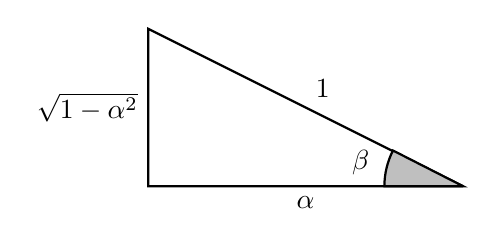
\begin{tikzpicture}[thick]
    \draw(4,0)
    -- (0,0) node[midway,below]{$\alpha$}
    -- (0,2) node[midway,left]{$\sqrt{1-\alpha^2}$} % node of point
    -- (4,0) node[midway,above right]{$1$};
    \draw[fill=lightgray, thick] (4,0)
    -- (3,0) arc (180:153:1cm) node at (2.7,0.3) {$\beta$}
    -- cycle;
\end{tikzpicture}

Nu is
\[ \sin (\arccos \alpha) = \sin \beta = \sqrt{1-\alpha^2}\,. \]
\subsection{Matrix in e-macht}\label{subsec:matrixInE-macht}
Deze definitie lijkt op de gewone definitie van $e^x$.
Als $A$ een matrix, dan geldt
\[ e^{At} \coloneqq \sum_{k=0}^\infty \frac{A^k t^k}{k!} \]
Voor $\displaystyle A = \matrix{0 & 1 \\ 1 & 0}$ geldt dan
\[ e^{At} =
\matrix{1 + \frac{t^2}{2!} + \frac{t^4}{4!} + \dots & t + \frac{t^3}{3!} + \dots \\
t + \frac{t^3}{3!} + \dots & 1 + \frac{t^2}{2!} + \frac{t^4}{4!} + \dots}
= \matrix{\cosh t & \sinh t \\ \sinh t & \cosh t}\]
\subsection{Imaginaire e-macht}\label{subsec:imaginaireE-macht}
\begin{align*}
    e^{ix} &= \cos x + i \sin x \\
    e^{-ix} &= \sin x + i \cos x
\end{align*}

    \section{Integralen}\label{sec:integralen}

    \begin{stelling}[Bell curve]
        \[ \int_{-\infty}^\infty e^{-\alpha x^2} \d x = \sqrt {\frac \pi \alpha}.\]
    \end{stelling}

    \begin{stelling}[Limiet door de integraal halen]
        Zij $\f_k,\f \: \reals^n \to \reals$, met $\lim_{k \to \infty} \f_k = \f$, dan
        \[ \f_k \text { \textbf{convergeert uniform} naar } \f \implies \lim \int \f_k = \int \lim \f_k = \int \f \,. \]
    \end{stelling}

    \section{Integreren}\label{sec:integreren}
    Onthoud:
\begin{align*}
    \int \frac{1}{\sin^2 u} \d u = \cotan u = \frac{1}{\tan u}
\end{align*}

\subsection{Integreren van even machten cosinus of sinus}\label{subsec:integrerenVanEvenMachtenCosinusOfSinus}

Mocht je iets willen integreren met $\cos^2$ dan volgt uit de verdubbelingsformules van sectie~\ref{gonioformules}
\begin{align*}
    \cos (2\alpha) &= \cos^2 \alpha - \sin^2 \alpha \\
    &=  \cos^2 \alpha + \cos^2 \alpha - \cos^2 \alpha - \sin^2 \alpha \\
    &= 2\cos^2 \alpha -1
\end{align*}
en evenzo voor $\sin^2 \alpha$.

\subsection{Partieel integreren}\label{subsec:partieelIntegreren}

\[
    \int_a^b f(x) g'(x) \d x = \big[f(x)g(x)\big]_a^b - \int_a^b f'(x) g(x) \d x
\]
dus kies $f$ en $g$ zodanig dat $f'(x)g(x)$ makkelijk integreert.

\subsubsection{Integeren van de (re\"ele) logaritme}

We nemen $f(x)=\ln x$ en $g'(x)=1$ zodat
\begin{align*}
    \int \ln x \cdot 1 \d x &= \int f(x)g'(x) \d x \\
    &= x \ln x - x \,.
\end{align*}

\subsection{Integreren door twee keer partieel}\label{subsec:integrerenDoorTweeKeerPartieel}

Als je een integraal van bijvoorbeeld de vorm
\[
    \int \sin t \cdot e^t \d t
\]
hebt, kun je opmerken dat als je een sinus twee keer integreert je weer een sinus
krijgt, en dus weer dezelfde integraal.
Dit kunnen we toepassen
door twee keer partieel te integreren (grenzen weggelaten voor de duidelijkheid).
\begin{align*}
    \int \sin t \cdot e^t \d t &= \sin t \cdot e^t - \int \cos t \cdot e^t \d t
    \quad \text{ met $f=\sin t$ en $g'=e^t$} \\
    &= \sin t \cdot e^t - \left( \cos t \cdot e^t - \int - \sin t \cdot e^t \d t \right)
    \quad \text{ met $f=\cos t$ en $g'=e^t$} \\
    &= ( \sin t - \cos t ) e^t -  \int \sin t \cdot e^t \d t
\end{align*}
Hieruit volgt dat
\[  \int \sin t \cdot e^t \d t = \frac{1}{2} ( \sin t - \cos t ) e^t\,. \]

\subsection{Integreren door breuksplitsen}\label{subsec:integrerenDoorBreuksplitsen}

We bekijken
\begin{align*}
    \int \frac{1}{u(1-u)} \d u &= \int \frac{A}{u} + \frac{B}{1-u} \d u \\
    &= \int \frac{A(1-u)+Bu}{u(1-u)} \d u
\end{align*}
waaruit volgt $A=B=1$ en dus
\[ \int \frac{1}{u(1-u)} \d u = \ln |u| + \ln |1-u|\,. \]
\subsection{Integreren door substitutie}\label{subsec:integrerenDoorSubstitutie}
We bekijken
\[ \int \sin t \cdot \cos t \cdot e^{\sin t} \d t\,. \]
Hierin zou je een functie en zijn afgeleide kunnen herkennen, namelijk
$\sin t$ en $\cos t$ waarbij een eventuele factor natuurlijk niet uitmaakt.
We substitueren $u = \sin t$, waaruit volgt $\d u = \cos t \d t$
zodat de integraal overgaat in
\[ \int u e^u \d u \]
wat we kunnen uitrekenen met partieel integreren.
Er volgt
\begin{align*}
    \int u e^u \d u &= u e^u - \int e^u \d u \\
    &= u e^u - e^u + c \\
    &= (\sin t -1) e^{\sin t} \,.
\end{align*}
Mochten er grenzen zijn, bijvoorbeeld
\[ \int_0^{\frac{\pi}{2}} \sin t \cdot \cos t \cdot e^{\sin t} \d t\,. \]
dan moeten we deze grenzen meesubstitueren, dus
\[ \int_{\sin 0}^{\sin \frac{\pi}{2}} u e^u \d u = 1\,. \]
\subsubsection{Integreren van oneven machten van de sinus}
We bekijken
\begin{align*}
    \int \sin^{2n+1} x \d x = \int \left( 1-\cos^2 x \right)^n \sin x \d x \,.
\end{align*}
We substitueren $u=\cos x$ dus $\d u = - \sin x \d x$.
Dan wordt dit
\begin{align*}
    \int -(1-u^2)^n \d u\,.
\end{align*}

    \section{Co\"ordinaten}\label{sec:coordinaten}
    Bij cilindercoordinaten is een extra \textbf{factor $\bm r$} verplicht als je integreert, bij bolcoordinaten $\rho^2 \sin \phi$
Om bolco\"ordinaten te onthouden, gebruik poolco\"ordinaten en druk $r$ uit in $\rho$ en $\phi$ met behulp van onderstaand driehoekje, zodat $r=\rho \sin \phi$, en vul deze in, in poolco\"ordinaten $r \cos \theta,r \sin \theta$ om $x$ en $y$ te krijgen.
Vind de $z$-co\"ordinaat op dezelfde manier zodat $z=\rho \cos \phi$.
Zie figuur~\ref{bolMMa} in de appendix om je gekozen co\"ordinaten te controleren met Mathematica.
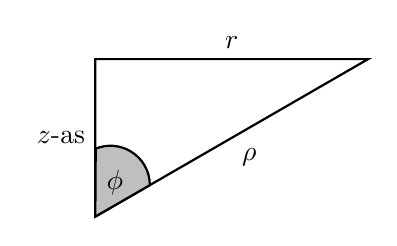
\begin{tikzpicture}[thick]
    \draw(0,0)
    -- (90:2cm) node[midway,left]{$z$-as}
    -- (30:4cm) node[midway,above]{$r$} % node of point
    -- (0,0) node[midway,below right]{$\rho$};
    \draw[fill=lightgray, thick] (0,0)
    -- (30:0.8cm) arc (0:112:0.5cm) node at (60:0.5cm) {$\phi$}
    -- cycle;
\end{tikzpicture}

    \section{Momenten uitrekenen}
    Om momenten makkelijk uit te rekenen kun je gebruik maken van kansgenererende functies in het geval van een discrete verdeling, of Laplacetransformaties voor een continue verdeling.

\subsection{Kansgenererende functie}

De kansgenererende functie is, voor een random variabele $X$,
\[
    P(z) = \E{z^X} = \sum_{k=0}^\infty \P{X=k} z^k.
\]
Deze kun je uitrekenen of vinden in een statistisch compendium.
Als je de afgeleide hiervan neemt, zie je dat
\[
    \frac{\d}{\d z} \E{z^X} = \E{Xz^{X-1}}
\]
dus
\[
    \E{X} = \eval{\frac{\d}{\d z} P(z)}_{z=1}.
\]
Evenzo,
\[
    \frac{\d^2}{\d z^2} P(z) = \E{X(X-1)z^{X-2}} = \E{X^2} - \E{X}
\]
dus
\[
    \E{X^2} = \eval{\frac{\d^2}{\d z^2} P(z)}_{z=1} + \E{X}.
\]
Enzovoorts voor het $k$-de moment.

\paragraph{Voorbeeld}
Zij $X \sim \Poi(\lambda)$, dan is 
\begin{align*}
    P(z) &= \E{z^X} \\
    &= \sumin z^k e^{-\lambda} \frac{\lambda^k}{k!} \\
    &= e^{-\lambda} \sumin \frac{(z\lambda)^k}{k!} \\
    &= e^{-\lambda} e^{z\lambda} \\
    &= e^{\lambda (z-1)}
\end{align*}
dus
\[
    \E{X} = \eval{\lambda e^{\lambda (z-1)}}_{z=1} = \lambda
\]
en
\[
    \E{X^2} = \eval{\lambda^2 e^{\lambda (z-1)}}_{z=1} + \E{X} = \lambda^2 + \lambda .
\]

\subsection{Momentgenererende functie}

De momentgenererende functie is een andere manier om een kansgenererende functie op te schrijven, namelijk
\[
    M_X(t) = \E{e^{tX}}
\]
dus als je de kansgenererende functie hebt vervang je $z=e^t$ en andersom.

\subsection{Laplacetransformatie}

Voor Laplacetransformaties geldt
\[
    \phi(s) = \int_{-\infty}^\infty e^{-st} f(t) \d t = \E{e^{-sX}}.
\]
Op dezelfde manier als bij kansgenererende functies kunnen we afgeleiden bepalen en daaruit de momenten halen.

\paragraph{Voorbeeld}

Zij $Z \sim \Norm(0,1)$, de Laplacetransformatie is
\begin{align*}
    \phi(s) &= \int_{-\infty}^\infty e^{-st} \frac{1}{\sqrt{2\pi}} e^{-\frac{t^2}{2}} \d t \\
    &= \int_{-\infty}^\infty \frac{1}{\sqrt{2 \pi}} e^{-st-\frac 1 2 t^2} \d t \\
    &= \int_{-\infty}^\infty \frac{1}{\sqrt{2 \pi}} e^{-\frac 1 2 (t^2 + 2st)} \d t \\
    &= \int_{-\infty}^\infty \frac{1}{\sqrt{2 \pi}} e^{- \frac 1 2 (t+s)^2 + \frac 1 2 s^2} \d t \\
    &= e^{\frac{s^2}{2}} \int_{-\infty}^\infty \frac{1}{\sqrt{2 \pi}} e^{- \frac 1 2 (t+s)^2} \d t \\
    &= e^{\frac{s^2}{2}}.
\end{align*}
We nemen de afgeleide
\[
    \frac{\d}{\d s} \phi (s) = \frac{\d}{\d s} \E{e^{-sZ}} = \E{-Z e^{-sZ}}
\]
dus 
\[
    \E{Z} = - \eval{\frac{\d}{\d s} \phi(s)}_{s=0}.
\]
In dit geval,
\[
    \eval{-s e^{\frac{s^2}{2}}}_{s=0} = 0
\]
en 
\[
    \E{Z^2} = \eval{-e^{\frac{s^2}{2}} - s^2 e^{\frac{s^2}{2}}}_{s=0} = -1.
\]
Merk verder op dat als $Y \sim \Norm(0,\sigma^2) = \sigma \Norm(0,1)$ dus $\E{Y^2} = \sigma^2 \E{Z^2}$, enzovoorts.


    \section{Determinant}\label{sec:determinant}
    \[
    \det{
        a & b & c \\
        d & e & f \\
        g & h & i \\
    }
    = a \det{e & f \\ h & i} - b \det{d & f \\ g & i} + c \det{d & e \\ g & h}
\]
\textbf{Let op het minteken!} Mintekens gaan als volgt:
\[
    \det{
        + & - & + \\
        - & + & - \\
        + & - & +
    }
\]

    \section{Inproduct/uitproduct}\label{sec:inproduct/uitproduct}
    \paragraph{Inproduct (dot product)}
\[ \x \bullet \bm \phi = \matrix{x \\ y \\ z} \bullet \matrix{\phi_1 \\ \phi_2 \\\phi_3} = x \phi_1 + y \phi_2 + z \phi_3 \]
\paragraph{Uitproduct (Vector/Cross product)}
\[ \matrix{x \\ y \\ z} \times \matrix{\phi_1 \\ \phi_2 \\\phi_3} = \matrix{y \phi_3 - \phi_2 z \\ z \phi_1 - \phi_3 x \\ x \phi_2 - \phi_1 y}  \]
eventueel te onthouden door (zie \LaTeX\ comments)
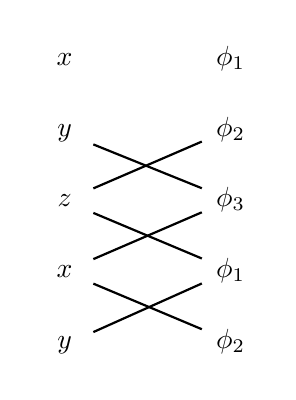
\begin{tikzpicture}[thick]
    \matrix (m) [matrix of math nodes, row sep = 1em, column sep = 4 em, minimum width=2em]
    {
    x & \phi_1 \\
    y & \phi_2 \\
    z & \phi_3 \\
    x & \phi_1 \\
    y & \phi_2 \\
    };
    \path[-stealth]
    (m-2-1) edge[-] (m-3-2) % y keer phi_3
    (m-2-2) edge[-] (m-3-1) % min phi_2 keer z,
    (m-3-1) edge[-] (m-4-2) % z keer phi_1
    (m-3-2) edge[-] (m-4-1) % min phi_3 keer x,
    (m-4-1) edge[-] (m-5-2) % x keer phi_2
    (m-4-2) edge[-] (m-5-1) % min phi_1 keer y
    ;
\end{tikzpicture}

    \section{Inhoud bol}\label{sec:inhoudBol}
    Inhoud is $\frac{4}{3} \pi r^3$, neem afgeleide voor oppervlakte.

    \section{Tussenwaarde/middelwaardestelling}\label{sec:tussenwaarde/middelwaardestelling}
    \begin{stelling}[\indx{Tussenwaardestelling}/Intermediate Value Theorem]

        Zij $a,b \in \reals,\ a<b,\
            f:[a,b]\to \reals \text{ continu}\,.
        $
        Zij $f(a)<y<f(b)$.
        Dan \[ \exists_{c\in(a,b)}:f(c)=y. \]
    \end{stelling}

    \begin{stelling}[\indx{Middelwaardestelling}/Mean Value Theorem]

        Zij $f\:[a,b] \to \reals$ continu, $f|_{(a,b)}$ differentieerbaar.
        Dan
        \[
            \exists_{c \in (a,b)} : f'(c) = \frac{f(b)-b(a)}{b-a}\,.
        \]
    \end{stelling}

    \section{Kwadraat afsplitsen}\label{sec:kwadraatAfsplitsen}
    Om een kwadratische vergelijking $x^2 + ax + b = 0$ op te lossen voor $x$ kunnen we in plaats van de abc-formule ook kwadraat afsplitsen.
    Let wel op dat de co\"efficient voor de $x^2$ een 1 is.
    \begin{align*}
        x^2 + a x + b &= 0 \\
        \left(x + \frac{1}{2} a\right)^2 - \left( \frac{1}{2}a \right)^2 &= - b \\
        \left(x + \frac{1}{2} a\right)^2 &= \left( \frac{1}{2}a \right)^2 - b \\
        x + \frac{1}{2} a &= \pm \sqrt{\left( \frac{1}{2}a \right)^2 - b} \\
        x &= -  \frac{1}{2} a \pm \sqrt{\left(\frac{1}{2}a \right)^2 - b}
    \end{align*}

    \newpage
    \section{Appendix}\label{sec:appendix}
    \begin{lstlisting}{language=mathematica}
        (* Transparent sphere *)
        pp = ParametricPlot3D[
        {Cos[u] Sin[v],
        Sin[u] Sin[v],
        Cos[v]},
        {u, 0, 2 Pi}, {v, 0, Pi}, Boxed -> False, Axes -> False,
        PlotStyle -> Opacity[0.05]];
        (* Part on the sphere (hold r) *)
        pp1 = ParametricPlot3D[
        {Cos[u] Sin[v],
        Sin[u] Sin[v],
        Cos[v]},
        {u, 0, 2 Pi}, {v, 0, Pi/6}, Axes -> False, Boxed -> False];
        (* Cone (hold v) *)
        pp2 = ParametricPlot3D[
        {r Cos[u] Sin[Pi/6],
        r Sin[u] Sin[Pi/6],
        r Cos[Pi/6]},
        {r, 0, 1}, {u, 0, 2 Pi}, Axes -> False, Boxed -> False];
        (* Combine the three parts *)
        Show[pp, pp1, pp2, ImageSize -> Large]
    \end{lstlisting}
    \begin{figure}[h!]
        \centering
        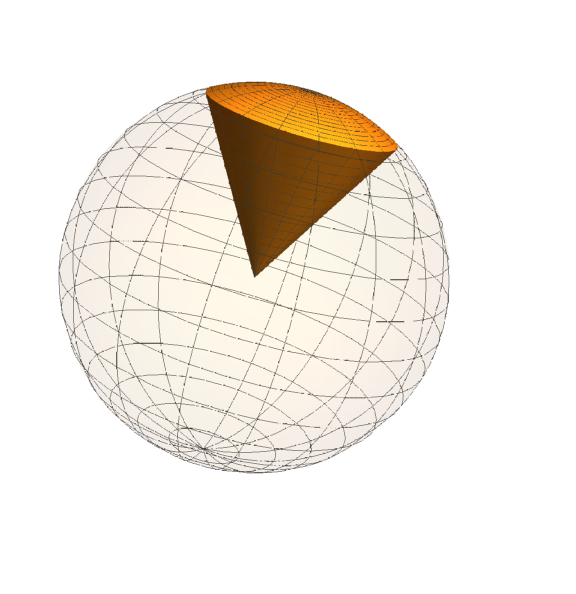
\includegraphics[width=.5\textwidth]{bol.png}
        \caption{Bol in Mathematica}\label{bolMMa}
    \end{figure}
\end{document}